\documentclass[12pt]{article}
\usepackage{url}
\usepackage{enumerate}
\usepackage{amssymb}
\usepackage{graphicx}
\usepackage[normalem]{ulem}
\oddsidemargin=-0.25in
\evensidemargin=-.25in
\textwidth=6.5in
\topmargin=-.55in
\textheight=9.2in

\renewcommand{\arraystretch}{1.3}
\renewcommand{\thefootnote}{\fnsymbol{footnote}}

\begin{document}

\pagestyle{empty}

\begin{center}

{\Large {\bf Clarifying Notes on Section 27.5:}}\\
\medskip
{\Large {\bf CA Naming Conventions}}\\
\bigskip
{\large {\bf Chaos and Fractals:}}\\
\medskip
{\bf {\large An Elementary Introduction}}\\
\bigskip
{ {\large David P.~Feldman}}\\
\smallskip
\today
\end{center}


%\noindent 
The convention for naming elementary CAs is entirely
standard.   In Section 27.5 I follow this convention.  So, for
example, the CA that I call 30 is the same CA that everyone else
would call 30.  

%\noindent 
However, I arrive at the conventional name by an
unconventional means, and this could possibly cause some confusion.
I think it will be most clear to illustrate this with an example.
First, I will show my way of setting up the equation that leads to a
CA name, and then I will show the way this is more typically done.  \\

\noindent {\bf {\large Method from Section 27.5}}\\


\begin{figure}[h]
\begin{center}
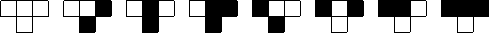
\includegraphics[width=120mm]{./ca_30_feldman.png}
\caption{CA Rule 30, shown as it would be in the text.  Note that the
  neighborhoods are listed, left-to-right, from the ``whitest'' to the
``blackest.''}
 \label{fig:ca_1}
\vspace{0mm}
\end{center}
\end{figure}

%\noindent 
Consider the CA shown in Fig.~\ref{fig:ca_1}.  Eight
three-site neighborhood are listed, and for each neighborhood the
output symbol is shown.  These output symbols are shown again in
Eq.~(\ref{eq:ca_30_1}): 
\begin{equation}
\label{eq:ca_30_1}
  \square \, \blacksquare \, \blacksquare \, \blacksquare \,
  \blacksquare \, \square \,\square \, \square \;\;. 
\end{equation}
Or, using $0$ for $\square$ and $1$ for $\blacksquare$, one writes:
\begin{equation}
 0 \, 1\, 1\, 1\, 1\, 0\, 0\, 0\;.
\end{equation}
This sequence of $0$'s and $1$'s is then converted into a base-$10$
number by viewing the sequence as a binary number,
\emph{left-to-right}:
\begin{eqnarray}
 0 \, 1\, 1\, 1\, 1\, 0\, 0\, 0\; &=& (0 \times 2^0) \, + \, 
    (1 \times 2^1) \, + \, (1 \times 2^2) \nonumber \\
& & \;\;+ \, (1 \times 2^3) \, + \, (1 \times 2^4) \, + \, (0 \times
 2^5) \nonumber \\
&   & \;\; + \, (0 \times 2^6) \, + \, (0 \times 2^7) \\
& = & 0 + 2 + 4 + 8 + 16 + 0 + 0 + 0 \\
& = & 30 \;.
\end{eqnarray}
Thus, the rule shown in Fig.~\ref{fig:ca_1} is rule 30. \\


\noindent {\bf {\large Standard Method}}\\

The approach described above correctly leads to designating the CA of
Fig.~\ref{fig:ca_1} as rule 30.  However, the path taken to do so is
not used by most other authors.  This section illustrates the more
standard approach.  The CA of Fig.~\ref{fig:ca_1} can also written as
shown in Fig.~\ref{fig:ca_2}.  Both figures show eight neighborhoods,
but the order in which these neighborhoods are opposite.  But both
figures show the same rule.  Each neighborhood's output is the same in
both figures---the neighborhoods just appear in a different location
in the list.  For a given initial condition, the rules shown in
Figs.~\ref{fig:ca_1} and \ref{fig:ca_2} would produce the exact same
space-time diagram, because the rules are exactly the same. 

\begin{figure}[h]
\begin{center}
\vspace{3mm}
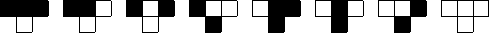
\includegraphics[width=120mm]{./ca_30_standard.png}
\caption{CA Rule 30, shown in the standard orientation.  Note that the
  neighborhoods are listed, left-to-right, from the ``blackest'' to the
``whitest.''}
 \label{fig:ca_2}
\vspace{0mm}
\end{center}
\end{figure}

The outputs for the rule shown in Fig.~\ref{fig:ca_2} are:
\begin{equation}
  \square \, \square \, \square \, \blacksquare \, \blacksquare \,
  \blacksquare \, \blacksquare \, \square \;.
\end{equation}
We now convert this to a binary number and then to base-$10$, but this
time we read \emph{right-to-left}.  That is, the smallest binary
digit is on the right, not the left:
\begin{eqnarray}
 0 \, 0\, 0\, 1\, 1\, 1\, 1\, 0\; &=& (0 \times 2^7) \, + \, 
    (0 \times 2^6) \, + \, (0 \times 2^5) \nonumber \\
& & \;\;+ \, (1 \times 2^4) \, + \, (1 \times 2^3) \, + \, (1 \times
 2^2) \nonumber \\
& & \;\; + \, (1 \times 2^1) \, + \, (0 \times 2^0) \\
&= & 0+0+0+16+8+4+2+0 \\
&= & 30 \;.
\end{eqnarray}
Thus, the rule shown in Fig.~\ref{fig:ca_2} is also rule 30. \\


\noindent {\bf {\large Conclusion}}\\

Both of the methods described above are correct, in that they yield
the standard name for a given rule.  However, the method referred to
above as the ``standard method'' is much more standard.  Almost any
other reference on CAs will use this approach.  I think the standard
method is probably better than my method, since in the standard method
the binary digits are read off in their usual order, with digits
increasing right to left.

I don't know why I chose the left-to-right method that I wrote in the
text.  I suppose at the time it seemed natural to me to do it this
way, and I didn't compare my discussion with any of the standard
texts; I just checked to make sure that it gave the right rule, which
is does.  

\end{document}
